\documentclass[UTF8,a4paper,11pt,fontset=windows]{ctexart}
\usepackage[margin=22mm,headheight=14pt]{geometry}
\usepackage{graphicx,booktabs,longtable,array,makecell,caption,needspace,tabularx,float}
\usepackage{amsmath,amssymb}
\usepackage[hidelinks]{hyperref}
\hypersetup{pdftitle={BP单因子测试报告},pdfsubject={三类股票池的回归、Rank IC、分层及适用域分析},pdfauthor={}}
\ctexset{section={format=\large\bfseries,beforeskip=16pt,afterskip=8pt},subsection={format=\normalsize\bfseries,beforeskip=12pt,afterskip=6pt}}
\linespread{1.18}
\setlength{\parskip}{3pt plus 1pt minus 1pt}
\setlength{\intextsep}{9pt plus 2pt minus 2pt}
\setlength{\textfloatsep}{12pt}
\setlength{\LTpre}{8pt}
\setlength{\LTpost}{5pt}
\setlength{\emergencystretch}{2em}
\captionsetup{font=small,skip=5pt,justification=raggedright,singlelinecheck=false}
\renewcommand{\arraystretch}{1.16}
\renewcommand{\topfraction}{0.95}
\renewcommand{\textfraction}{0.05}
\renewcommand{\floatpagefraction}{0.8}
\makeatletter
\setlength{\@fptop}{0pt}
\setlength{\@fpsep}{12pt}
\setlength{\@fpbot}{0pt plus 1fil}
\makeatother
\raggedbottom
\widowpenalty=10000
\clubpenalty=10000
\begin{document}
\pagestyle{plain}
\begin{center}
{\LARGE\bfseries BP单因子测试报告}\par
\vspace{6pt}
{\large 三类股票池的收益区分能力与适用边界}\par
\vspace{5pt}
{\small 方法版本0.5\quad 2026年10月26日}
\end{center}
\begin{abstract}
本文检验正且有限历史PB倒数所构成的BP因子，预期高BP对应较高下期收益。采用月末信号、下一交易日收盘换仓、行业与规模控制、加权最小二乘回归（WLS）、等级信息系数（Rank IC）及扣教材成本的等权分层，沪深300、中证500与全部 A 股共同评价2007-02至2026-01归属的228个完整持有期。全部 A 股平均Rank IC为0.0566，正向月份162/228；五层年化净收益由4.55\%递增至20.98\%，多空年化13.00\%，Q5相对内部基准的算术年化超额5.31\%。指数池方向相同而强度较弱。行业共同窗口中Q5在19/30个可比行业排名第一；房地产、钢铁等行业为负超额，综合行业样本不足。2025年正IC与负多头超额并存，低市值域的排序关系更强。结论是保留BP作为后续研究候选，观察时变性与行业边界；历史版本修订、估值近似及简化成本使本结果不能直接解释为严格PIT或实盘可实现收益。
\end{abstract}
\noindent\textbf{关键词：}账面市值比；单因子测试；Rank IC；行业中性化；分层回测。

\section{研究背景与因子简介}
单因子测试是多因子研究的起点，其作用是检验一个信号能否在同一期股票之间区分后续收益，并判断这种关系的稳定性和适用范围。本报告按照课程附录，以回归、Rank IC与等权分层三类证据评价BP，再考察年度、行业和市值域的差异。研究问题是：控制行业与规模后，较高BP是否仍对应较高下期收益，以及这一关系在哪些范围内失效。

BP属于估值类因子。较高BP意味着账面权益相对市场定价较高，可能反映较低估值，也可能包含较高经营风险。本文先给出操作定义，再检验正向假说；预期方向在计算绩效之前确定。

\begin{table}[H]\centering
\caption*{\textbf{表1　因子定义与默认方向}}
\small\renewcommand{\arraystretch}{1.2}
\begin{tabularx}{\linewidth}{@{}p{26mm}X@{}}\toprule
项目 & 定义 \\ \midrule
因子 & 账面市值比（Book-to-Price，BP） \\
经济概念 & 账面权益与市场价值之比 \\
实际计算 & $\mathrm{BP}_{i,t}=1/\mathrm{PB}_{i,t}$，仅使用正且有限的历史PB \\
源字段 & 课程离线估值表的\texttt{pb}；供应商当前定义为总市值除以“净资产减其他权益工具” \\
单位与频率 & 无量纲比值；交易月末收盘后取值 \\
预期方向 & 正向。Q1为低中性化残差层，Q5为高中性化残差层；十层时Q10最高 \\
无效值 & 缺失、零、负和无穷PB均不填补；这是定义域限制，不属于去极值 \\
控制与分域 & 控制规模使用对数总市值；WLS权重和市值分域使用流通市值，源市值单位为万元 \\
\bottomrule\end{tabularx}
\end{table}

实际检验依赖供应商历史日度PB，不能直接等同于已自行重构的、当时可获得且未经修订的账面权益序列。已有字段定义和有限财务样本支持这一操作口径，但严格的逐版本时点可得性（point-in-time，PIT）尚不能证明。

高BP后续取得较高收益，可能与错误定价修正或风险补偿有关；资产减值、盈利能力下降和持续经营风险也可能构成“价值陷阱”。这些解释并不互斥，本文的观察性检验不能识别其因果机制。非线性和适用域分析用于限定结论，而非根据结果改选因子或反转方向。

\section{截面诊断}
基础合格池U已应用历史ST/PT和入场资格筛选；F为U中可构造BP的股票；S为F中行业与市值控制变量可用的分析样本。覆盖率统一定义为F/U。

\subsection{一级行业分布}
\Needspace{185mm}
\begin{figure}[H]\centering
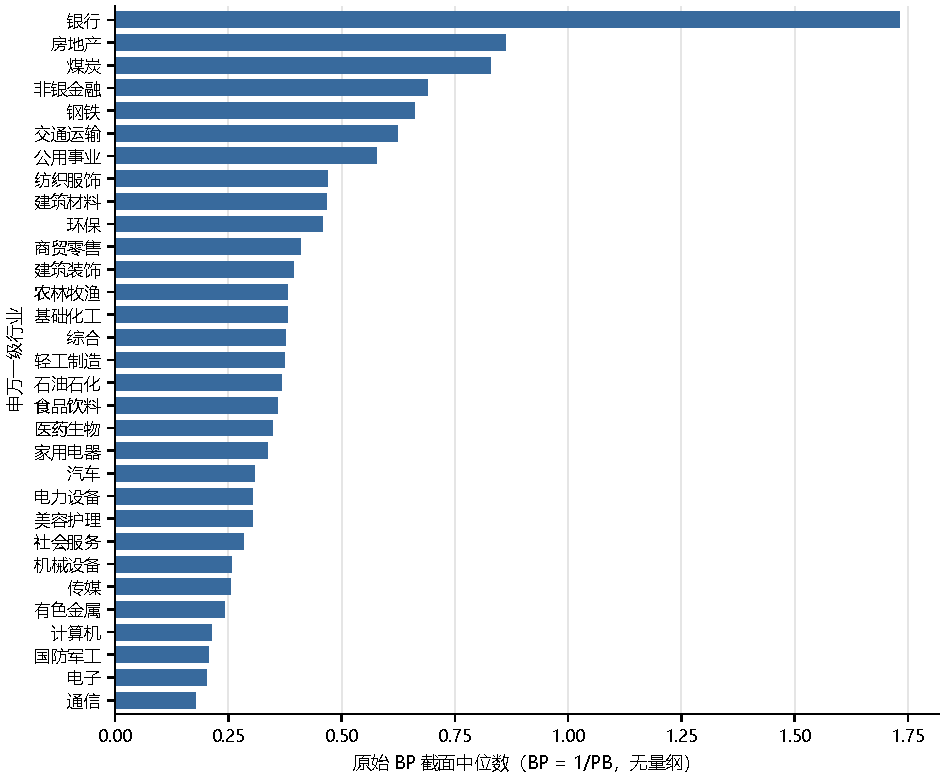
\includegraphics[width=.8\linewidth]{figures/industry_median.pdf}
\caption*{\textbf{图A　最新截面的行业BP中位数}\ 2026-01-30；使用正且有限PB的F样本；覆盖31个一级行业。横轴为原始BP，不是中性化残差。}
\end{figure}

最新截面共5273只F股票、31个一级行业。银行BP中位数为1.732，通信为0.177，前者约为后者的9.8倍。房地产和煤炭也处于较高区间。这种行业差异支持在比较股票之前控制行业；不能把银行高BP本身解释为银行股票具有更高预测收益。综合行业在本截面仅15只，仍展示中位数，但不据此认定其行业分层可靠。

\Needspace{115mm}
\subsection{BP与规模的关系}
\Needspace{85mm}
\begin{figure}[H]\centering
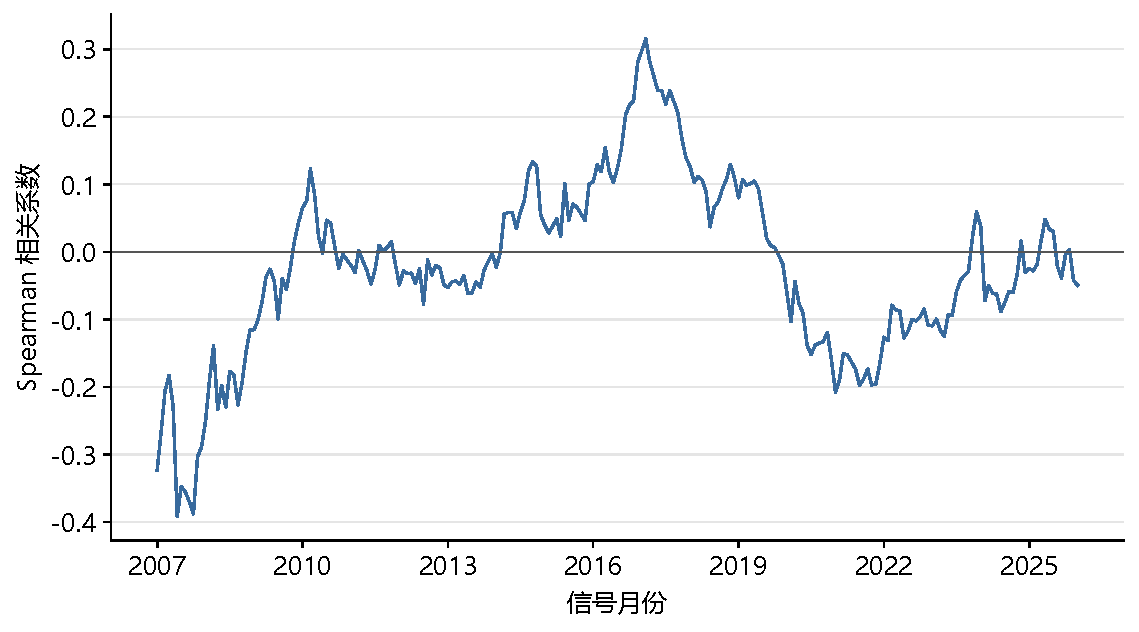
\includegraphics[width=.87\linewidth]{figures/size_correlation.pdf}
\caption*{\textbf{图B　原始BP与对数总市值的截面相关}\ 2007-01至2026-01，共229个信号月；逐月计算Spearman相关，未按未来收益筛选。}
\end{figure}

229/229个信号截面均可计算，相关系数均值为-0.0228；与均值同为负号的月份为136/229（59.39\%），正号为93/229。均值较小并不表示每月都与规模无关，图中方向曾发生反转。因此保留逐期规模控制，且不把中性化后的低相关倒写为原始BP无规模关联。

\Needspace{100mm}
\subsection{覆盖度与样本流转}
\Needspace{85mm}
\begin{figure}[H]\centering
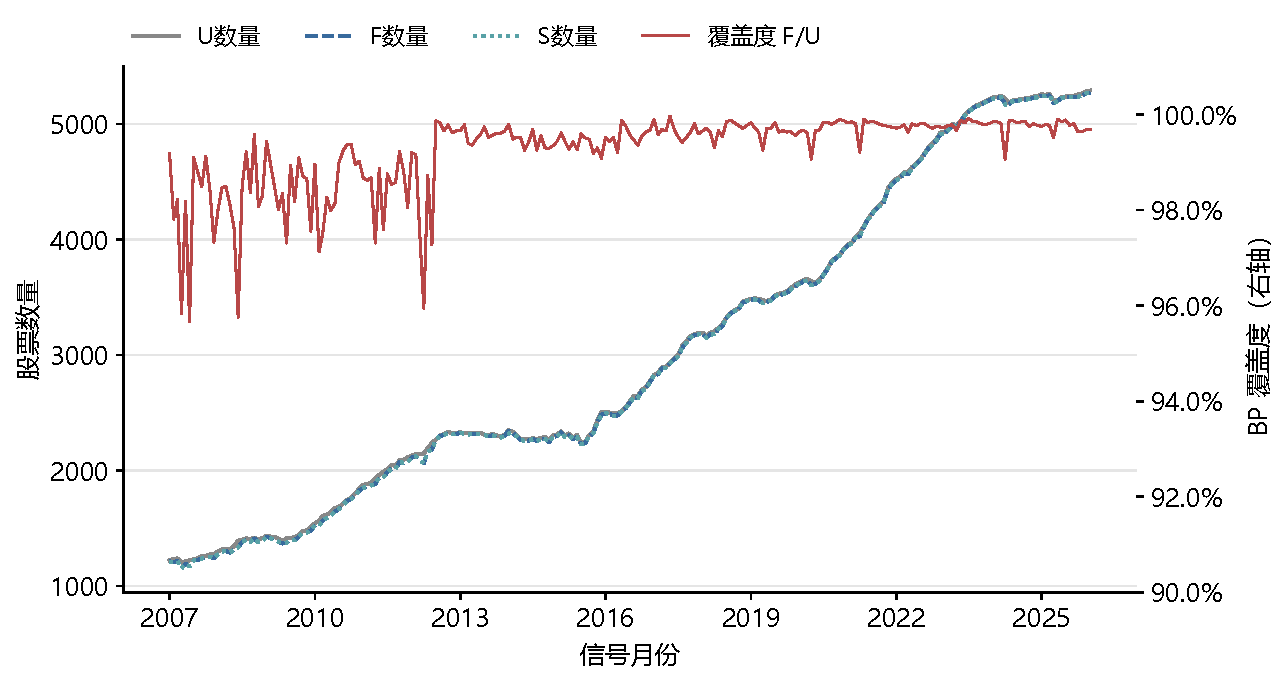
\includegraphics[width=.87\linewidth]{figures/D1.pdf}
\caption*{\textbf{图D1　合格样本与BP覆盖度}\ 全部 A 股；229个信号月。数量读左轴，覆盖率F/U读右轴；收益检验只使用其中228个完整持有期。}
\end{figure}

全部 A 股各月F/U介于95.66\%与99.97\%。最新截面U=5,290、F=S=5,273，覆盖度为99.68\%。229期累计U与F之差为3,602个股票期观测，其中估值整行缺失2,660、PB字段缺失942、非有限0、零值0、负值0。缺失不能统一解释为负净资产；ST/PT和入场不合格已在U之前过滤，不进入覆盖率分母。覆盖度较高仅支持数据可用性，不等于预测有效性。


\section{数据与方法}
\subsection{研究窗口与历史样本}
三类股票池共同使用2007-01至2025-12信号月，共228期。实际建仓从2007-02-01收盘开始，最后退出为2026-02-02收盘；持有期按建仓月份归属2007-02至2026-01。2026-01-30仅用于最新完整截面的分布诊断，其计划退出日超出行情截止，未进入绩效。

全部 A 股沿用课程沪深京人民币权益证券覆盖，包含库内境内上市中国存托凭证（CDR）；北交所自2021-11-15开市后纳入。历史生命周期、指数成员、行业和ST/PT状态均按有效日期匹配，不用当前名单或市值排名代替历史指数池。入场资格采用下一交易日收盘可交易口径，全天或收盘仍停牌者剔除，日内临停后已恢复收盘交易者可保留。

三个池分别在S上进行预处理和分层，之后才接入未来响应Y。完整窗口的全部 A 股共有686,280个股票--期。原始8,011个退出端点不足中，7,936项按停牌与公司行为规则估值，58项依据事先公告在最后实际交易日退出后持有零利息现金，17项按合并对价估值。其中两项承接A股尚未上市，采用已确认的换股权利估值延续。处理后未解决端点为0，原持仓与计划持有期未因未来可观测性改变。

行业使用历史生效事件，保留早期分类，不把现行分类倒填。229个诊断月合计87个F股票--期缺行业，按预先确定的控制变量规则从S排除。有限流通市值异常已按公司股本事件修正。这些修复支持当前历史字段研究，不构成全市场财报、行业与股本版本的严格PIT重建。

\subsection{默认测试设定}
普通最小二乘法（OLS）用于因子中性化，加权最小二乘法（WLS）用于收益回归；无风险收益率（RF）设为0。

\begin{table}[H]\centering
\caption*{\textbf{表2　统一参数与评价定义}}
\small\renewcommand{\arraystretch}{1.18}
\begin{tabularx}{\linewidth}{@{}p{25mm}X@{}}\toprule
项目 & 本报告采用的设定 \\ \midrule
频率与时点 & 月末生成信号；下一交易日收盘换仓，至下一次换仓日收盘结束 \\
去极值 & 截面中位数$\pm5\times\mathrm{MAD}$，MAD为绝对离差的中位数 \\
回归暴露 & 去极值后的标准分数（Z-score），截面标准差分母为$n$（ddof=0） \\
中性化 & 去极值BP对截距、$\ln(\text{总市值})$及行业哑变量作OLS，取残差 \\
WLS & 下期收益对标准化BP、对数总市值和行业回归；目标函数权重$w_i=\sqrt{\text{流通市值}_i}$ \\
Rank IC & 冻结的中性化残差与下期个股收益的Spearman相关 \\
分层 & 五层等人数、层内等权；并列按证券代码稳定排序；十层与分域复用相同残差 \\
成本 & 教材只数换手，首期为1；每层扣$0.004\times TO$；多空两腿分别扣费 \\
内部基准 & 同期全部实际分层股票的等权毛收益，不另扣换手成本 \\
外部指数 & 沪深300、中证500价格指数；共同入/退出端点，不含分红 \\
时间统计 & RF=0；时间序列标准差分母为$n-1$；ICIR不年化 \\
缺值与缺期 & 不填补因子；无法合理估值的持仓不重分权；缺月不补零或拼接年化 \\
\bottomrule\end{tabularx}
\end{table}

回归检验线性条件关联，Rank IC检验截面排序，分层则检验离散组合的成本后收益。三者使用相同日期与形成样本，但权重和关系形状不同，不要求数值等价。负的中性化残差仍是有效因子值。退化截面、设计矩阵不满秩或样本不足均显式记录；本次三池主窗口均可完整评价。

个股收益由同一原始代码复权尺度的入、退出估值构造。教材只数换手与多空净收益分别为
\begin{align}
TO_{q,t}&=1-\frac{|S_{q,t}\cap S_{q,t-1}|}{|S_{q,t}|},\qquad TO_{q,1}=1,\\
r^{LS,net}_t&=r^{gross}_{5,t}-r^{gross}_{1,t}-0.004TO_{5,t}-0.004TO_{1,t}.
\end{align}
这一近似不模拟权重漂移、完整再平衡、成交冲击或融资借券。多空净值按$\prod_t(1+r^{LS,net}_t)$计算，沿用教材资本口径，不另除以2。

对连续完整月度净收益$r_t$，复合年化收益率（CAGR）为$[\prod_t(1+r_t)]^{12/n}-1$，夏普比率为$\sqrt{12}\,\bar r/s_r$。设月超额$e_t=r_{q,t}^{net}-r_{b,t}^{gross}$，算术年化超额为$12\bar e$，信息比率（IR）为$\sqrt{12}\,\bar e/s_e$。净值均含期初1；最大回撤为净值相对历史峰值的最小变化，报告为非正数。超额最大回撤对相对净值$NAV_q/NAV_b$作相同计算。

C1的信息系数比率（ICIR）为月IC均值除以样本标准差，不乘$\sqrt{12}$。截面$t$使用课程常规WLS方差估计，未作稳健标准误调整；其均值和绝对值均值不构成因子收益时间序列均值的显著性检验。D2与D3分别累加IC和回归系数，不复利。D6在每个连续12期窗口内计算层收益复利与基准收益复利之差，前11期为空。

\subsection{分域比较与解释窗口}
D9在全部 A 股同一形成样本与残差上重分十层。D10每月先按流通市值等人数分为低、中、高三域，再在域内按同一残差十等分。C4在历史一级行业内部重分五层，不重新估计行业内规模斜率。分域基准均为域内实际分层股票的等权毛收益；控制变量缺失者不为构造基准重新纳入。这是相对附录“因子非空”定义的明确资格限制。

C4每期至少25只，D10每域至少50只，并检验不同因子取值数。C4共同信号窗在查看收益前冻结为2021-07至2025-12，共54期，实际入场2021-08-02、退出2026-02-02。综合行业只有12期达到门槛，保留不足行，不拼接年化或进入同窗排名。

时间解读采用三个连续日历块：2007-02至2013-12、2014-01至2020-12、2021-01至2026-01，均按持有期起始月归属。这些分段仅作描述，不用于调整主窗口或额外推断显著性。内部基准与分层的成本待遇不同，外部价格指数与个股复权收益的分红口径也不同，后文分别解释。

\section{主结果与适用域}
\subsection{三类股票池的回归与Rank IC}
\begingroup\small\setlength{\tabcolsep}{4pt}
\begin{table}[H]\centering
\caption*{\textbf{表C1(a)　回归法汇总}}
\begin{tabular*}{\textwidth}{@{\extracolsep{\fill}}llrrrr@{}}\toprule
股票池 & 因子 & $|t|$均值 & $|t|>2$占比 & $t$均值 & \makecell{因子收益均值\\（\%/月）} \\ \midrule
沪深300 & BP & 2.106 & 101/228 (44.30\%) & 0.531 & 0.34 \\
中证500 & BP & 1.898 & 87/228 (38.16\%) & 0.466 & 0.25 \\
全部 A 股 & BP & 4.729 & 160/228 (70.18\%) & 1.757 & 0.40 \\
\bottomrule\end{tabular*}
\par\smallskip\raggedright\footnotesize 各池均有228期。回归系数对应一单位标准化BP暴露；表中是截面$t$统计量。\end{table}
\endgroup

三池的平均回归系数均为正。全部 A 股绝对t均值4.729，绝对t>2共160/228期，t均值1.757；沪深300、中证500的t均值分别为0.531和0.466。全部 A 股t>2为100期、t<$-$2为60期，WLS系数为正的月份为126/228，少于下表中IC为正的162/228，排序证据的逐月一致性强于线性回归证据。

\begingroup\small\setlength{\tabcolsep}{4pt}
\begin{table}[H]\centering
\caption*{\textbf{表C1(b)　Rank IC汇总}}
\begin{tabular*}{\textwidth}{@{\extracolsep{\fill}}llrrrr@{}}\toprule
股票池 & 因子 & IC均值 & IC标准差 & ICIR & $IC>0$占比 \\ \midrule
沪深300 & BP & 0.0366 & 0.1279 & 0.286 & 134/228 (58.77\%) \\
中证500 & BP & 0.0350 & 0.1056 & 0.332 & 145/228 (63.60\%) \\
全部 A 股 & BP & 0.0566 & 0.1028 & 0.550 & 162/228 (71.05\%) \\
\bottomrule\end{tabular*}
\par\smallskip\raggedright\footnotesize 时间序列标准差使用$n-1$分母；ICIR未年化。\end{table}
\endgroup

全部 A 股平均Rank IC为0.0566，162/228期为正，ICIR为0.550；沪深300与中证500分别为0.0366、0.0350。三池方向与平均回归系数一致，全部 A 股的强度最高。三池使用同一窗口，强度差异来自股票池的成员范围与截面规模。

\subsection{五层排序与多空收益}
\begingroup\small\setlength{\tabcolsep}{4pt}
\begin{table}[H]\centering
\caption*{\textbf{表C2(a)　五层年化净收益}}
\begin{tabular*}{\textwidth}{@{\extracolsep{\fill}}llrrrrrr@{}}\toprule
股票池 & 因子 & Q1 & Q2 & Q3 & Q4 & Q5 & \makecell{递增相邻\\层数/4} \\ \midrule
沪深300 & BP & 2.22 & 3.78 & 3.14 & 7.31 & 10.40 & 3/4 \\
中证500 & BP & 5.64 & 7.61 & 8.99 & 10.16 & 13.50 & 4/4 \\
全部 A 股 & BP & 4.55 & 8.71 & 14.00 & 17.75 & 20.98 & 4/4 \\
\bottomrule\end{tabular*}
\par\smallskip\raggedright\footnotesize 收益单位为\%，为复合年化净收益（CAGR）。三池层序与年化收益的Spearman相关分别为0.900、1.000、1.000。每池228期，所有层均已扣教材成本。\end{table}
\endgroup

全部 A 股五层年化净收益从4.55\%依次升至20.98\%，4/4个相邻层递增，层序与年化收益Spearman为1，呈严格单调。中证500同样4/4递增；沪深300为3/4，仅Q3略低于Q2。三池排序均支持正向BP假说。成本拖累很小：建仓后Q1、Q5的平均月度只数换手为13.6\%与11.4\%，按双边千分之四折合年化约0.65与0.55个百分点；中间三层换手较高，为24.4\%至28.7\%。

\begingroup\small\setlength{\tabcolsep}{4pt}
\begin{table}[H]\centering
\caption*{\textbf{表C2(b)　多空绩效与多头超额}}
\begin{tabular*}{\textwidth}{@{\extracolsep{\fill}}lrrrrr@{}}\toprule
股票池 & \makecell{多空年化\\（\%）} & 夏普 & \makecell{最大回撤\\（\%）} & 多空月胜率 & \makecell{Q5年化超额\\（百分点）} \\ \midrule
沪深300 & 5.28 & 0.470 & -47.50 & 121/228 (53.07\%) & 3.41 \\
中证500 & 5.09 & 0.513 & -22.94 & 121/228 (53.07\%) & 2.79 \\
全部 A 股 & 13.00 & 1.150 & -15.66 & 136/228 (59.65\%) & 5.31 \\
\bottomrule\end{tabular*}
\par\smallskip\raggedright\footnotesize 夏普、回撤和胜率对应多空；Q5年化超额为相对内部等权毛基准的算术年化差额。\end{table}
\endgroup

全部 A 股扣双腿成本后的多空年化为13.00\%、夏普1.150、最大回撤$-$15.66\%。两个指数股票池多空年化约5\%，回撤更深：沪深300为$-$47.50\%（2018-12至2021-07），中证500为$-$22.94\%（2018-10至2021-06），都对应下文2019至2021年的失效期。按第3.2节的分解，全部 A 股多空净收益的算术年化值为12.89个百分点，其中多头部分5.31个百分点、空头部分7.59个百分点，低BP端的落后贡献约59\%。

\Needspace{70mm}
\subsection{排序关联与线性系数的时间路径}
\begin{figure}[H]\centering
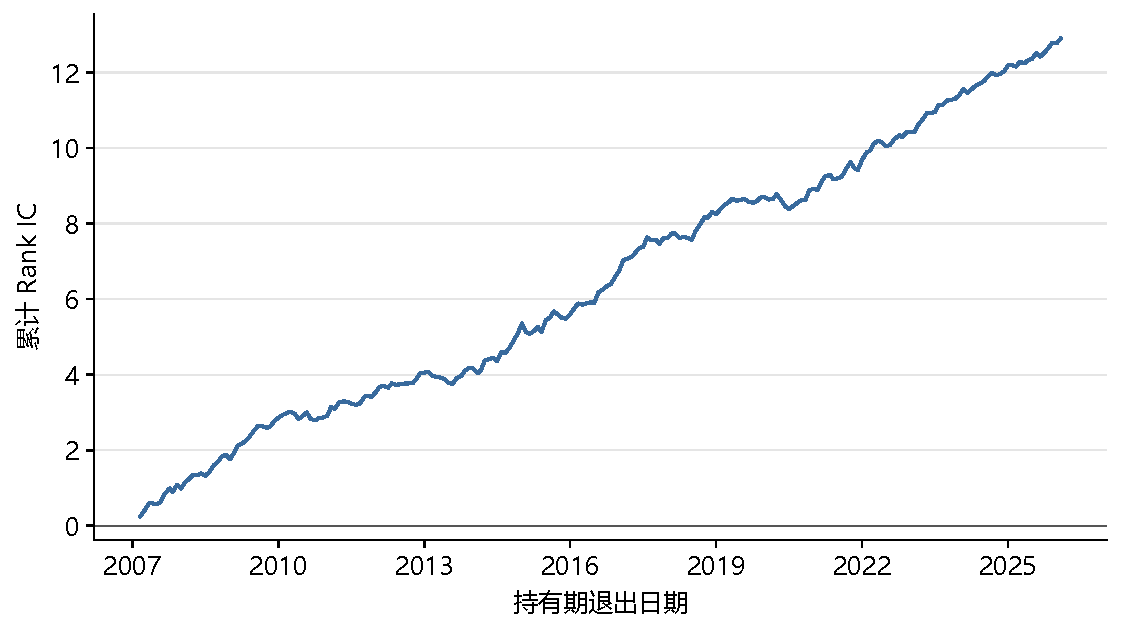
\includegraphics{figures/D2.pdf}
\caption*{\textbf{图D2　Rank IC算术累计}\ 全部 A 股，228期；逐期相加，纵轴是Rank IC算术累计。横轴为持有期归属月份。}
\end{figure}

三个日历块的平均Rank IC分别为0.0502（2007-02至2013-12，83期）、0.0567（2014-01至2020-12，84期）、0.0652（2021-01至2026-01，61期），均为正且逐块上升。2010、2013年全年平均Rank IC接近零（0.0038与0.0090），累计曲线在2010-04至2010-12（9个月）和2013-02至2013-09（8个月）短暂走平，总体仍呈上行趋势，期间也有短暂回落。

\Needspace{70mm}
\begin{figure}[H]\centering
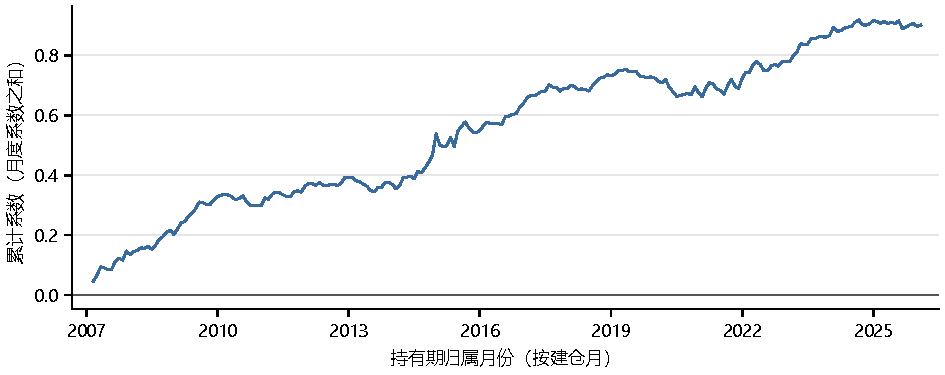
\includegraphics{figures/D3.pdf}
\caption*{\textbf{图D3　回归因子系数算术累计}\ 全部 A 股，228期；标准化BP的月度系数逐期相加，系数为小数，0.01对应1\%。横轴为持有期归属月份。}
\end{figure}

228期回归系数累计为0.9017，三个日历块分别贡献0.3690、0.3073、0.2253，正向累计分布在整个样本期。累计系数在2019-04达到0.7546后回落，2021-01降至最低（回落0.0929），2022-03创新高，低于前高34个月；2024-08以后至样本末端未再创新高（17个月）。同期累计Rank IC低于前高的区间都不超过7个月：2019年后线性斜率走弱，总体排序仍持续累积。

\Needspace{90mm}
\subsection{绝对净值、相对财富与滚动超额}
\begin{figure}[H]\centering
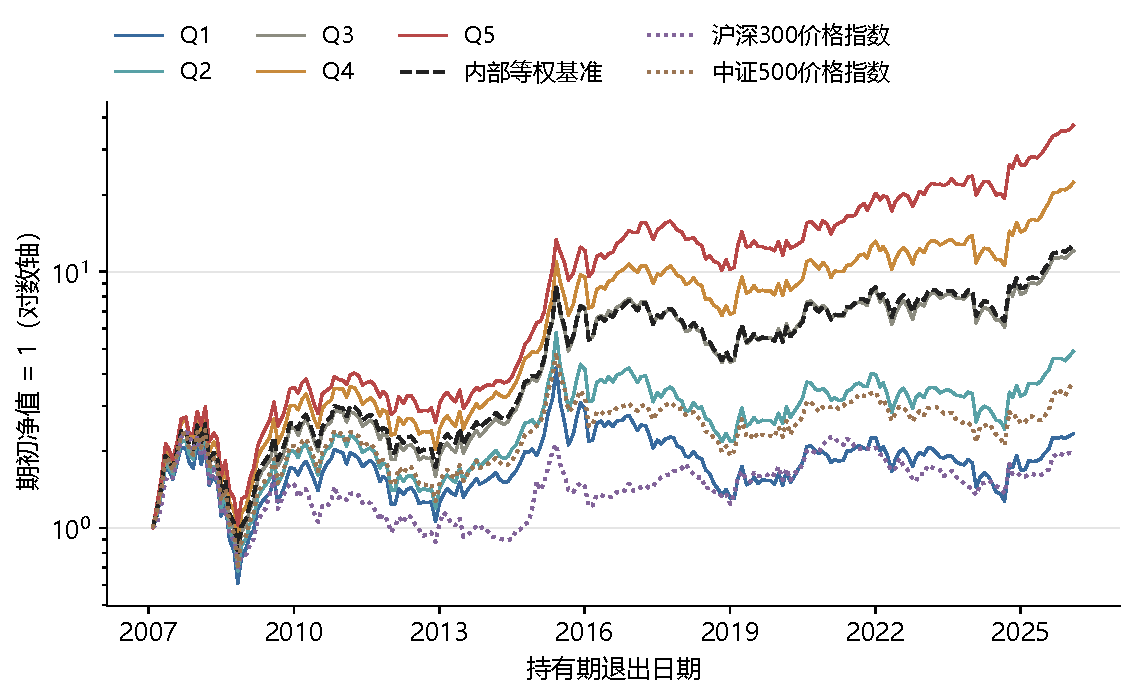
\includegraphics{figures/D4.pdf}
\caption*{\textbf{图D4　五层组合、内部基准与价格指数净值}\ 期初为1，实际端点2007-02-01至2026-02-02；纵轴为倍数，对数刻度；横轴为持有期归属月份。分层扣费，内部基准未扣费，外部价格指数不含分红。}
\end{figure}

同样从1开始，期末Q5净值为37.276，内部基准为12.739，Q1为2.330；沪深300和中证500价格指数分别为1.923与3.712。五层净值按层序拉开，Q5的期末财富约为内部基准的2.9倍、Q1的16倍；Q5期间最大回撤为$-$65.45\%。Q3与内部基准几乎重合（期末12.049与12.739）。

\Needspace{80mm}
\begin{figure}[H]\centering
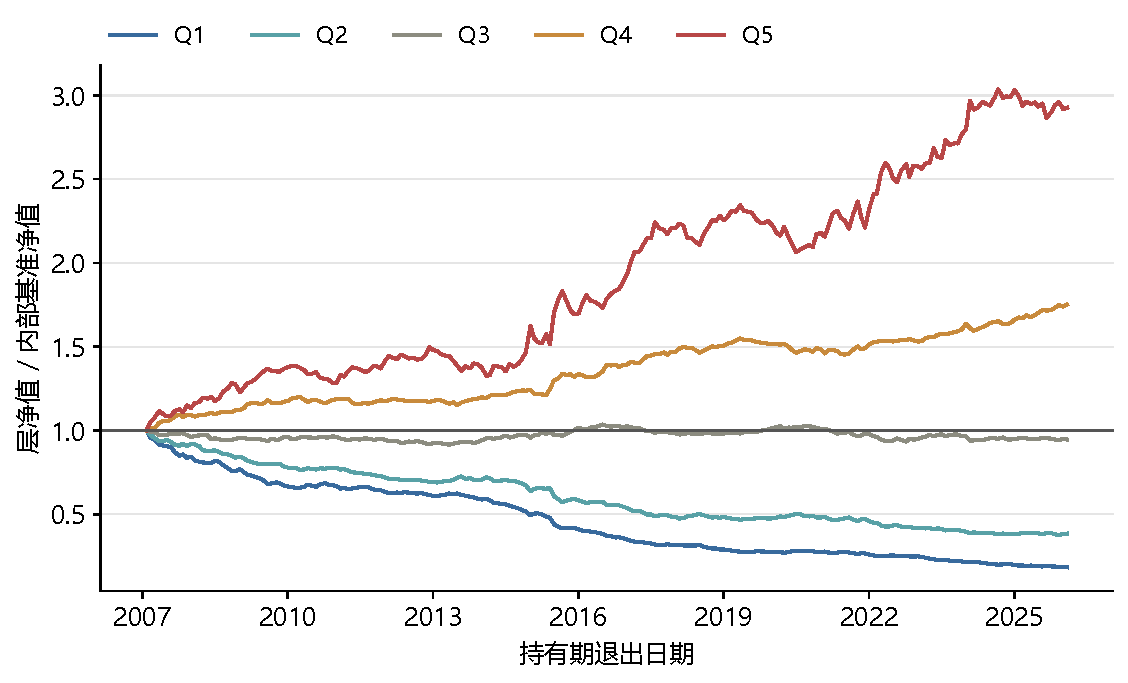
\includegraphics{figures/D5.pdf}
\caption*{\textbf{图D5　五层净值除以内部基准净值}\ 全部 A 股，228期；相对净值大于1表示截至当期的层净财富高于内部基准。阴影为Q5相对净值连续12个月以上低于此前高点的区间。}
\end{figure}

期末Q5/基准为2.926，Q4为1.751，Q3为0.946，各层相对财富按层序排列。Q5相对净值连续12个月以上低于此前高点的区间共六段（以下均计低于前高的观察月数）。最深的一段在2019-04见顶后回撤11.92\%（低点2020-06），2021-09创新高，期间28个观察月低于前高；其次是2012-11见顶后的24个月（最深$-$11.34\%）和2010-01见顶后的19个月（$-$7.37\%）；2015-08与2017-07见顶后另有12至13个月的较浅回撤（$-$7.54\%、$-$5.99\%）。2024-08见顶后的一段持续到样本末端，期末比前高低3.60\%。

\Needspace{90mm}
\begin{figure}[H]\centering
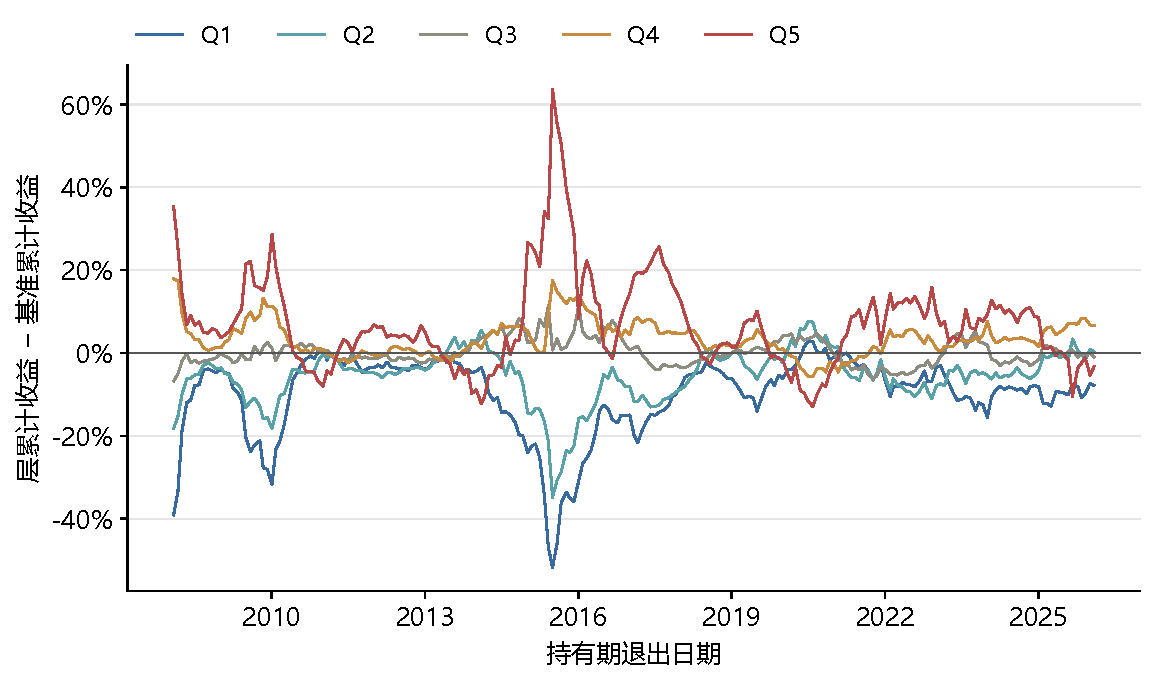
\includegraphics{figures/D6.pdf}
\caption*{\textbf{图D6　滚动12个月复利超额收益}\ 全部 A 股；层净收益复利减基准毛收益复利，纵轴以百分数显示差额；前11个月为空，共217个重叠窗口。阴影为Q5连续为负不少于6个端点的区间；横轴为窗口末月的持有期归属月份。}
\end{figure}

图D6把长期累计优势展开到具体窗口，分段均值见下表。

\begingroup\small\setlength{\tabcolsep}{4pt}
\begin{table}[H]\centering
\caption*{\textbf{表D6附表　各层滚动12个月超额的分段均值}}
\begin{tabular*}{\textwidth}{@{\extracolsep{\fill}}lrrrrrr@{}}\toprule
持有期归属区间 & 有效点 & Q1 & Q2 & Q3 & Q4 & Q5 \\ \midrule
2007-02至2013-12 & 72 & $-$7.75 & $-$5.12 & $-$0.71 & 2.57 & 5.08 \\
2014-01至2020-12 & 84 & $-$13.61 & $-$6.53 & 2.18 & 4.26 & 8.97 \\
2021-01至2026-01 & 61 & $-$7.80 & $-$4.69 & $-$1.36 & 3.19 & 6.55 \\
\bottomrule\end{tabular*}
\par\smallskip\raggedright\footnotesize 单位为百分点。分段按滚动端点归属，窗口可跨分段边界，相邻窗口重叠11期。\end{table}
\endgroup

Q5滚动超额为正的点为161/217（74.19\%）。按连续为负不少于6个端点的判据，失效区间有四段：2010-06至2011-03（10个端点，最低$-$7.99\%）、2013-04至2014-06（15个，$-$12.18\%）、2019-09至2021-01（17个，$-$12.91\%）和2025-06至2026-01（8个，$-$10.44\%）。最后一段持续到样本末端，末值为$-$3.26\%。三个分段的Q5均值均为正（5.08、8.97、6.55个百分点），五层分段均值也都按层序排列，失效期之外的超额足以弥补失效期的回落。

\Needspace{80mm}
\begin{figure}[H]\centering
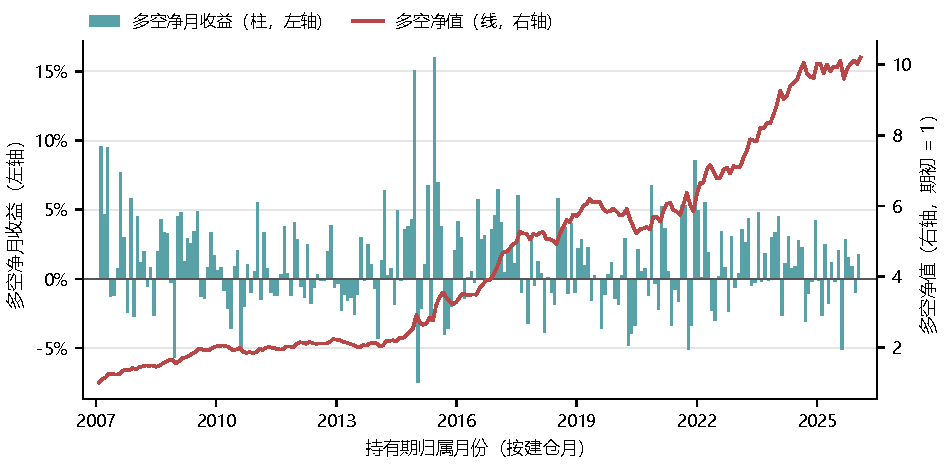
\includegraphics{figures/D7.pdf}
\caption*{\textbf{图D7　多空月收益与累计净值}\ 月收益读左轴，复利净值读右轴；Q5毛收益减Q1毛收益后扣两腿成本。两轴刻度相互独立；横轴为持有期归属月份。}
\end{figure}

多空正收益为136/228个月（59.65\%），期末净值10.197。最差月为2015-01（$-$7.49\%），最好月为2015-06（15.99\%），均按持有期起始月份归属。多空净值的最大回撤$-$15.66\%发生在2019-04至2020-06，2021-09回到前高，与D5、D6识别的失效期一致；此后至样本末端净值由6.194升至10.197。

\Needspace{80mm}
\subsection{五层与十层的风险调整表现}
\begin{figure}[H]\centering
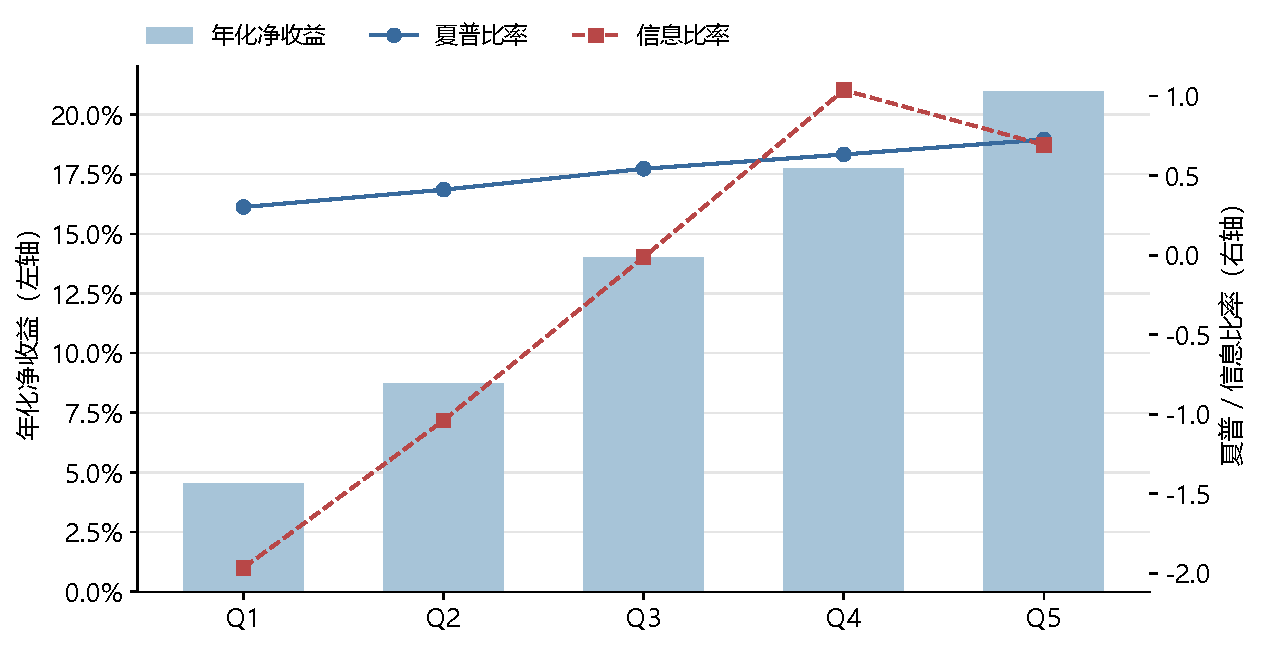
\includegraphics{figures/D8.pdf}
\caption*{\textbf{图D8　五层收益与风险调整指标}\ 年化净收益为柱，夏普与IR为双线；RF=0，时间序列标准差的分母为$n-1$；共228期。}
\end{figure}

五层年化净收益和夏普均逐层递增，Q5夏普为0.727。Q4的IR为1.038，高于Q5的0.693；相对月胜率分别为60.09\%和53.07\%（分母均为228期），超额最大回撤分别为$-$6.19\%和$-$11.92\%。Q5收益最高，Q4的信息比率最高、超额最大回撤最浅。

\Needspace{80mm}
\begin{figure}[H]\centering
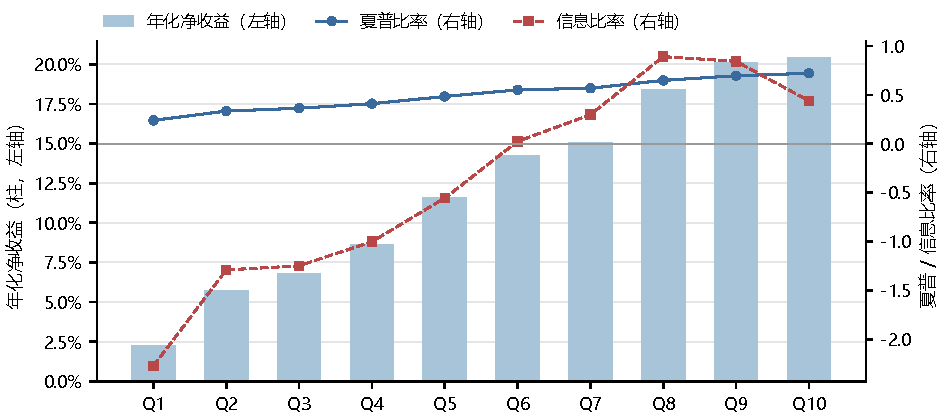
\includegraphics{figures/D9.pdf}
\caption*{\textbf{图D9　十层收益与风险调整指标}\ 保持全部 A 股样本、预处理及成本不变，只将五层改为十层；共228期。}
\end{figure}

十层年化净收益9/9对相邻层递增，层序秩相关1.000，单调性在更细分组下依然成立。Q9与Q10分别为20.12\%、20.43\%，最高尾部的收益增益已很小。Q10的算术年化超额为4.66个百分点，与Q9的4.92个百分点接近，但IR由0.843降至0.439，超额最大回撤由$-$9.21\%扩大到$-$17.61\%，相对月胜率由54.82\%降至49.12\%。最高中性化残差层的超额波动明显上升，与价值陷阱假说相容，但不能据此识别其成因。

\Needspace{80mm}
\subsection{流通市值三域}
\begin{figure}[H]\centering
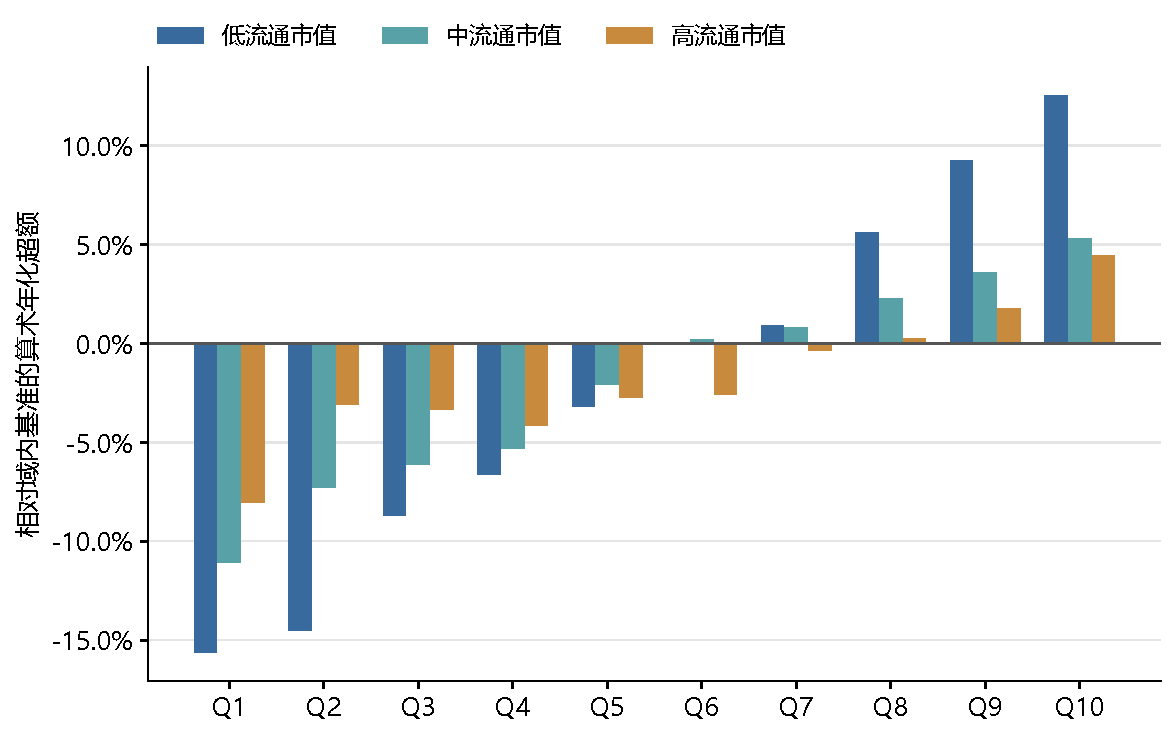
\includegraphics{figures/D10.pdf}
\caption*{\textbf{图D10　三市值域内十层年化超额}\ 各域先按流通市值形成，再按全部 A 股残差分层；年化超额为相对域内等权毛基准的算术年化超额。}
\end{figure}

低、中市值域的层序平滑，高市值域Q2至Q4出现倒序。附表列出域内股票数量、两端超额与Q10信息比率。

\begingroup\small\setlength{\tabcolsep}{4pt}
\begin{table}[H]\centering
\caption*{\textbf{表D10附表　市值域的样本量与两端超额}}
\begin{tabular*}{\textwidth}{@{\extracolsep{\fill}}lrrrrr@{}}\toprule
流通市值域 & 每期只数范围 & Q1年化超额 & Q10年化超额 & Q10信息比率 & 递增相邻层数/9 \\ \midrule
低 & 384--1755 & $-$15.64 & 12.54 & 0.905 & 9/9 \\
中 & 383--1755 & $-$11.08 & 5.31 & 0.622 & 9/9 \\
高 & 384--1755 & $-$8.03 & 4.44 & 0.387 & 7/9 \\
\bottomrule\end{tabular*}
\par\smallskip\raggedright\footnotesize 超额为相对域内基准（等权毛收益）的算术年化超额，单位为百分点；三域均有228期。每月先按流通市值三等分，再在各域内按同一份全部 A 股残差十等分。\end{table}
\endgroup

三域均有228期，Q10算术年化超额分别为12.54、5.31、4.44个百分点，信息比率为0.905、0.622、0.387；低、中市值域的十层超额均9/9递增，高市值域为7/9。BP的排序关系随市值上升而减弱，在低流通市值域最强。高市值域只有Q8至Q10为正超额，Q10信息比率不到低市值域的一半，大市值股票中的BP效应集中在最高几层。低市值域Q10建仓后平均月度只数换手约21.2\%，提示需关注成本影响，实际交易成本敏感性尚未评估。各域在BP及控制变量均有效的S样本中划分，因此域内BP完整率为100\%，不代表原始合格池的分域覆盖率；市值分界按每月等人数划分，先分域、再按全样本残差分层。

\clearpage
\subsection{一级行业内部比较}
\begingroup\small\setlength{\tabcolsep}{4pt}
\begin{longtable}{lrrrrrr}
\caption*{\textbf{表C4(a)　行业内五层的Q5绩效}}\\
\toprule
一级行业 & 有效期 & \makecell{年化超额\\（百分点）} & 夏普 & IR & \makecell{超额回撤\\（\%）} & \makecell{相对月\\胜率（\%）} \\ \midrule
\endfirsthead
\caption*{表C4(a)　行业内五层的Q5绩效（续）}\\\toprule
一级行业 & 有效期 & \makecell{年化超额\\（百分点）} & 夏普 & IR & \makecell{超额回撤\\（\%）} & \makecell{相对月\\胜率（\%）} \\ \midrule
\endhead
\midrule\multicolumn{7}{r}{续下页}\\\endfoot
\bottomrule\endlastfoot
家用电器 & 54/54 & 17.93 & 1.164 & 1.556 & $-$5.48 & 64.81 \\
美容护理 & 54/54 & 14.39 & 0.562 & 0.665 & $-$18.96 & 55.56 \\
电力设备 & 54/54 & 12.72 & 0.767 & 1.418 & $-$7.80 & 66.67 \\
食品饮料 & 54/54 & 10.59 & 0.555 & 1.276 & $-$4.64 & 61.11 \\
电子 & 54/54 & 10.01 & 0.824 & 1.084 & $-$7.42 & 57.41 \\
社会服务 & 54/54 & 9.84 & 0.887 & 0.874 & $-$8.34 & 61.11 \\
计算机 & 54/54 & 9.57 & 0.749 & 1.081 & $-$6.38 & 66.67 \\
医药生物 & 54/54 & 8.25 & 0.555 & 1.043 & $-$5.45 & 70.37 \\
农林牧渔 & 54/54 & 7.58 & 0.585 & 1.016 & $-$5.13 & 55.56 \\
纺织服饰 & 54/54 & 7.19 & 0.822 & 0.872 & $-$6.49 & 57.41 \\
交通运输 & 54/54 & 7.04 & 0.980 & 0.769 & $-$8.81 & 50.00 \\
非银金融 & 54/54 & 6.82 & 0.488 & 1.131 & $-$4.30 & 66.67 \\
机械设备 & 54/54 & 6.32 & 0.950 & 0.717 & $-$7.62 & 64.81 \\
国防军工 & 54/54 & 6.04 & 0.572 & 0.755 & $-$5.98 & 59.26 \\
公用事业 & 54/54 & 5.08 & 0.734 & 0.651 & $-$6.62 & 50.00 \\
石油石化 & 54/54 & 4.95 & 0.872 & 0.433 & $-$16.15 & 53.70 \\
银行 & 54/54 & 2.72 & 0.709 & 0.369 & $-$11.39 & 55.56 \\
环保 & 54/54 & 2.43 & 0.423 & 0.333 & $-$9.01 & 53.70 \\
有色金属 & 54/54 & 2.38 & 0.824 & 0.216 & $-$11.42 & 53.70 \\
汽车 & 54/54 & 2.07 & 0.798 & 0.191 & $-$16.61 & 51.85 \\
通信 & 54/54 & 1.60 & 0.896 & 0.162 & $-$15.17 & 55.56 \\
基础化工 & 54/54 & 1.45 & 0.562 & 0.189 & $-$9.65 & 53.70 \\
建筑装饰 & 54/54 & 0.80 & 0.645 & 0.072 & $-$18.77 & 48.15 \\
轻工制造 & 54/54 & 0.68 & 0.529 & 0.096 & $-$14.05 & 48.15 \\
传媒 & 54/54 & 0.52 & 0.765 & 0.038 & $-$16.68 & 53.70 \\
煤炭 & 54/54 & $-$0.09 & 0.527 & $-$0.006 & $-$24.71 & 48.15 \\
建筑材料 & 54/54 & $-$1.53 & 0.354 & $-$0.141 & $-$25.57 & 46.30 \\
商贸零售 & 54/54 & $-$4.69 & 0.440 & $-$0.626 & $-$17.40 & 42.59 \\
房地产 & 54/54 & $-$6.39 & 0.105 & $-$0.586 & $-$40.77 & 33.33 \\
钢铁 & 54/54 & $-$6.75 & 0.010 & $-$0.749 & $-$28.33 & 37.04 \\
综合 & 12/54 & --- & --- & --- & --- & --- \\
\end{longtable}
\noindent\footnotesize 共同信号窗为2021-07至2025-12（54期，持有期归属2021-08至2026-01），按年化超额降序。年化超额为算术年化超额；夏普对应Q5，IR、超额回撤和胜率相对行业内部基准（等权毛收益）。完整行业胜率分母均为54；综合行业不计算共同窗口绩效。\par
\endgroup

在2021-07至2025-12信号窗口（持有期归属2021-08至2026-01）的30个可比行业中，Q5年化超额为正25/30，BP在多数行业内有效。家用电器最高，为17.93个百分点；房地产与钢铁分别为$-$6.39和$-$6.75个百分点，商贸零售与建筑材料为$-$4.69和$-$1.53个百分点，煤炭接近零。综合行业未形成完整共同窗口，绩效留空。

\begingroup\small\setlength{\tabcolsep}{4pt}
\begin{longtable}{lrrlr}
\caption*{\textbf{表C4(b)　行业内收益排序与样本量}}\\
\toprule
一级行业 & \makecell{每期最少\\股票数} & \makecell{Q5收益\\名次} & 层收益排序 & 层序相关$\rho$ \\ \midrule
\endfirsthead
\caption*{表C4(b)　行业内收益排序与样本量（续）}\\\toprule
一级行业 & \makecell{每期最少\\股票数} & \makecell{Q5收益\\名次} & 层收益排序 & 层序相关$\rho$ \\ \midrule
\endhead
\midrule\multicolumn{5}{r}{续下页}\\\endfoot
\bottomrule\endlastfoot
家用电器 & 74 & 1 & $Q_5>Q_3>Q_4>Q_2>Q_1$ & 0.900 \\
美容护理 & 27 & 1 & $Q_5>Q_4>Q_2>Q_3>Q_1$ & 0.900 \\
电力设备 & 257 & 1 & $Q_5>Q_4>Q_3>Q_2>Q_1$ & 1.000 \\
食品饮料 & 105 & 1 & $Q_5>Q_4>Q_3>Q_2>Q_1$ & 1.000 \\
电子 & 317 & 1 & $Q_5>Q_4>Q_3>Q_2>Q_1$ & 1.000 \\
社会服务 & 65 & 1 & $Q_5>Q_4>Q_3>Q_2>Q_1$ & 1.000 \\
计算机 & 271 & 1 & $Q_5>Q_4>Q_3>Q_1>Q_2$ & 0.900 \\
医药生物 & 374 & 1 & $Q_5>Q_4>Q_3>Q_2>Q_1$ & 1.000 \\
农林牧渔 & 87 & 1 & $Q_5>Q_4>Q_2>Q_3>Q_1$ & 0.900 \\
纺织服饰 & 98 & 1 & $Q_5>Q_4>Q_2>Q_3>Q_1$ & 0.900 \\
交通运输 & 120 & 1 & $Q_5>Q_3>Q_4>Q_2>Q_1$ & 0.900 \\
非银金融 & 77 & 1 & $Q_5>Q_4>Q_2>Q_3>Q_1$ & 0.900 \\
机械设备 & 418 & 1 & $Q_5>Q_4>Q_3>Q_2>Q_1$ & 1.000 \\
国防军工 & 108 & 1 & $Q_5>Q_4>Q_3>Q_2>Q_1$ & 1.000 \\
公用事业 & 112 & 1 & $Q_5>Q_4>Q_3>Q_2>Q_1$ & 1.000 \\
石油石化 & 42 & 1 & $Q_5>Q_2>Q_3>Q_1>Q_4$ & 0.300 \\
银行 & 40 & 1 & $Q_5>Q_3>Q_4>Q_1>Q_2$ & 0.800 \\
环保 & 103 & 1 & $Q_5>Q_4>Q_3>Q_2>Q_1$ & 1.000 \\
有色金属 & 118 & 2 & $Q_3>Q_5>Q_2>Q_4>Q_1$ & 0.500 \\
汽车 & 217 & 2 & $Q_3>Q_5>Q_4>Q_2>Q_1$ & 0.700 \\
通信 & 98 & 1 & $Q_5>Q_4>Q_3>Q_1>Q_2$ & 0.900 \\
基础化工 & 311 & 2 & $Q_4>Q_5>Q_3>Q_2>Q_1$ & 0.900 \\
建筑装饰 & 134 & 3 & $Q_4>Q_3>Q_5>Q_2>Q_1$ & 0.700 \\
轻工制造 & 122 & 2 & $Q_4>Q_5>Q_2>Q_3>Q_1$ & 0.800 \\
传媒 & 120 & 2 & $Q_4>Q_5>Q_2>Q_3>Q_1$ & 0.800 \\
煤炭 & 33 & 3 & $Q_1>Q_4>Q_5>Q_2>Q_3$ & -0.200 \\
建筑材料 & 72 & 3 & $Q_4>Q_3>Q_5>Q_1>Q_2$ & 0.600 \\
商贸零售 & 90 & 4 & $Q_3>Q_4>Q_2>Q_5>Q_1$ & 0.300 \\
房地产 & 88 & 5 & $Q_3>Q_4>Q_2>Q_1>Q_5$ & -0.100 \\
钢铁 & 43 & 4 & $Q_3>Q_4>Q_1>Q_5>Q_2$ & 0.100 \\
综合 & 15 & --- & 样本不足 & --- \\
\end{longtable}
\noindent\footnotesize 收益排序按各层年化净收益从高到低排列；相关系数是层序与年化收益的Spearman相关。共30个完整行业，综合行业保留不足行。\par
\endgroup

Q5在19/30个可比行业排名第一，在24/30个行业进入前二，行业内排序整体稳健。层序方向相反的行业为煤炭（$\rho=-0.200$，Q1收益最高）和房地产（$\rho=-0.100$，Q5收益最低）；商贸零售与钢铁的Q5名次为第4。石油石化Q5虽排名第一，层序相关只有0.300。美容护理每期最少仅27只，接近25只门槛。综合行业只有12/54期达到门槛，列为样本不足。

\Needspace{60mm}
\section{分年度表现与稳健性}
\subsection{分年度表现}
\begingroup\small\setlength{\tabcolsep}{4pt}
\begin{longtable}{lrrrrrrr}
\caption*{\textbf{表C3　全部 A 股分年度表现}}\\
\toprule
年份 & 月数 & \makecell{多空\\收益} & \makecell{多空月\\胜率} & \makecell{Q5\\收益} & \makecell{内部基准\\收益} & \makecell{多头\\超额} & 平均IC \\ \midrule
\endfirsthead
\caption*{表C3　全部 A 股分年度表现（续）}\\\toprule
年份 & 月数 & \makecell{多空\\收益} & \makecell{多空月\\胜率} & \makecell{Q5\\收益} & \makecell{内部基准\\收益} & \makecell{多头\\超额} & 平均IC \\ \midrule
\endhead
\midrule\multicolumn{8}{r}{续下页}\\\endfoot
\bottomrule\endlastfoot
2007* & 11 & 37.39 & 63.64 & 184.68 & 150.96 & 33.71 & 0.0896 \\
2008 & 12 & 12.36 & 66.67 & -53.13 & -56.76 & 3.63 & 0.0650 \\
2009 & 12 & 30.89 & 83.33 & 164.05 & 135.40 & 28.66 & 0.0918 \\
2010 & 12 & -8.44 & 50.00 & 6.87 & 14.86 & -7.99 & 0.0038 \\
2011 & 12 & 12.38 & 58.33 & -26.52 & -33.32 & 6.80 & 0.0523 \\
2012 & 12 & 6.39 & 41.67 & 10.94 & 6.09 & 4.84 & 0.0431 \\
2013 & 12 & -4.65 & 25.00 & 17.91 & 26.76 & -8.85 & 0.0090 \\
2014 & 12 & 38.12 & 75.00 & 74.61 & 47.88 & 26.73 & 0.0993 \\
2015 & 12 & 12.71 & 50.00 & 91.24 & 82.89 & 8.35 & 0.0212 \\
2016 & 12 & 28.65 & 75.00 & 17.53 & 3.19 & 14.33 & 0.0952 \\
2017 & 12 & 22.51 & 66.67 & 0.72 & -11.80 & 12.51 & 0.0723 \\
2018 & 12 & 10.22 & 58.33 & -28.71 & -30.16 & 1.45 & 0.0526 \\
2019 & 12 & 2.37 & 66.67 & 28.81 & 30.54 & -1.73 & 0.0369 \\
2020 & 12 & -2.70 & 50.00 & 16.54 & 18.97 & -2.44 & 0.0192 \\
2021 & 12 & 11.54 & 50.00 & 32.26 & 23.75 & 8.51 & 0.0645 \\
2022 & 12 & 11.76 & 66.67 & -1.22 & -10.78 & 9.56 & 0.0602 \\
2023 & 12 & 25.24 & 66.67 & 18.04 & 8.82 & 9.22 & 0.0813 \\
2024 & 12 & 13.13 & 66.67 & 10.51 & 1.94 & 8.56 & 0.0659 \\
2025 & 12 & -0.17 & 50.00 & 37.61 & 43.00 & -5.39 & 0.0495 \\
2026* & 1 & 1.80 & 100.00 & 3.83 & 3.52 & 0.31 & 0.1173 \\
\end{longtable}
\noindent\footnotesize 收益与胜率单位为\%，多头超额单位为百分点。年度按持有起始月归属；*为部分年度，报告实际累计收益，不向全年外推。胜率分母为该行月数。\par
\endgroup

2007年仅11期、2026年仅1期，为实际累计收益。18个完整年度中，多空收益为正14/18年，复利口径的多头超额为正13/18年，两条年度序列的相关系数为0.94，总体同步；多空不利年份为2010、2013、2020、2025。按第3.3节的判据，空头端驱动的年份为2015、2018和2019年：三年的多头部分为$-$0.21、2.09、$-$1.41个百分点，空头部分为14.42、8.12、3.95个百分点；2023年空头部分占64\%，接近该界限。2015年复利多头超额为8.35个百分点，算术多头部分为$-$0.21个百分点，差异来自逐月求和与复利运算的不同，而非仅由基准上涨放大造成。2025年多空接近零（$-$0.17\%），两端算术贡献4.32与$-$4.18个百分点相抵，但不能直接相加为年度复利收益；同年平均Rank IC为0.0495，排序关联仍在，最高层却跑输基准。

本报告的稳健性证据来自三方面：三个股票池方向一致（第4.1、4.2节）；三个日历块的平均Rank IC均为正（第4.3节）；五层与十层的年化净收益排序一致（第4.5节）。去极值方法敏感性见第5.2节，IC衰减与样本外检验留待后续研究。

% BEGIN WINSOR SENSITIVITY 20261029
\Needspace{85mm}
\subsection{去极值方法敏感性}
\begingroup\small\setlength{\tabcolsep}{3pt}
\begin{table}[H]\centering
\caption*{\textbf{表S1　去极值方法敏感性}}
\begin{tabular*}{\textwidth}{@{\extracolsep{\fill}}lrrrrr@{}}\toprule
去极值方案 & \makecell{Rank IC\\均值} & ICIR & \makecell{回归因子收益\\均值（\%/月）} & \makecell{多空年化\\净收益（\%）} & \makecell{Q5算术年化超额\\（百分点）} \\ \midrule
MAD5 & 0.0566 & 0.550 & 0.40 & 13.00 & 5.31 \\
MAD3 & 0.0565 & 0.522 & 0.40 & 12.34 & 4.80 \\
1\%/99\%分位数缩尾 & 0.0563 & 0.563 & 0.38 & 13.32 & 5.55 \\
\bottomrule\end{tabular*}
\par\smallskip\raggedright\footnotesize 全部 A 股，228期；仅改变去极值方法，其余设定及输入S样本不变。ICIR未年化；多空为扣除双腿成本后的CAGR；Q5超额为相对原内部等权毛收益基准的算术年化超额。分位点采用线性插值。差值按未舍入结果计算。
\end{table}
\endgroup

本节完成去极值敏感性分析，比较MAD5、MAD3与1\%/99\%分位数缩尾；IC衰减与样本外检验仍留待后续。表S1中，三种方案的平均回归因子收益均为正（0.38\%至0.40\%/月），平均Rank IC为0.0563至0.0566，方向一致；ICIR为0.522至0.563。相对MAD5，MAD3与分位数方案的多空年化净收益分别变化$-$0.66、+0.32个百分点，Q5算术年化超额分别变化$-$0.51、+0.25个百分点。三种方案五层年化净收益均随层号递增。按可加总的算术年化口径，MAD3毛多空下降0.55个百分点，双腿成本增加0.01个百分点，净收益下降主要来自毛收益变化。由此，原结论的正向关联与分层单调性得到支持，但收益幅度仍依赖去极值选择，不能称为完全稳健。

% END WINSOR SENSITIVITY 20261029

\section{结论}
结论为“保留”。三类证据方向一致：三池回归系数与平均Rank IC均为正，成本后五层收益在全部 A 股和中证500中严格单调。全部 A 股平均Rank IC为0.0566，多空年化13.00\%，Q5相对内部基准的算术年化超额为5.31个百分点。BP最适用于全部 A 股，在低流通市值域最强；两个指数股票池方向相同、强度较弱。BP可以作为后续多因子研究的估值类候选因子。

BP的效果具有时变性。Q5相对内部基准有两段较深的失效：2019-04见顶后回撤11.92\%、29个月后创新高，2012-11见顶后回撤11.34\%、低于前高24个观察月。样本末端处于新的失效期：Q5相对净值低于2024-08高点，滚动12个月超额自2025-06起连续为负，累计回归系数自2024-08后未创新高。行业层面，在2021-07至2025-12窗口内，房地产、钢铁等5个行业的Q5跑输各自基准。多空收益约59\%来自低BP端的落后；只做多时，可获得的主要是5.31个百分点的多头超额。

三类证据衡量的对象不同：WLS反映加权线性斜率，Rank IC反映全截面排序，等权高层组合只使用尾部股票并扣费。因此正IC、正回归与个别年份Q5的弱超额可以同时出现，D8、D9中高层IR的回落也说明高期望收益与低超额波动需要分开评价。

进入多因子合成时须注意共线风险。原始BP与对数总市值的逐月相关在$-$0.392至0.316之间，并有四段持续两年以上的同号期；行业间BP中位数相差近10倍（图A）。合成前应先检验BP与规模、行业以及EP等其他估值或质量因子的相关冗余，并在新的时间窗与可执行成本下确认其增量。

数据与成本口径有三点说明：历史PB与行业取自当前可得的历史版本，未作逐版本时点重建；停牌、退市与合并端点按已声明政策估值；成本采用教材只数换手，不含冲击成本与融券约束。多空均值的异方差与自相关稳健（HAC）检验、行业多重检验校正与样本外评估可作为后续工作。

\appendix
\section{资料与复现说明}
本报告唯一实证运行标识为\path{bp-v05-20261026-main}，方法版本0.5，研究源码提交\path{38a5369}。本LaTeX工程复用该运行的锁定汇总，不重新估计因子模型。\path{source-data/}保存制表与制图所需的汇总CSV，\path{tables/}和\path{figures/}保存可直接编译的表格与矢量图，\path{sections/}为可编辑正文。

方法依据为课程\textit{main\_student.pdf}附录书197--200页（PDF211--214页），成本、净值及IC定义另参考书177--183页（PDF191--197页）。本轮已重新阅读原PDF文字和渲染页。BP作为贯穿估值样例采用月末截面；未将ROE等财务质量因子的每年三次截面规则混用于本报告。

课程实现复用\path{qfbook.factor.single_test}的MAD、标准化、中性化、设计矩阵和双腿扣费；形成/响应分离、冻结WLS暴露、完整日期索引与期初净值由项目适配实现。数据修复证据、测试与逐项来源见主项目的预检和验收记录。原始股票库、证券级形成暴露和持仓留在本地，未纳入本工程。本文没有引用未经核实的外部论文，也没有把教材EP样例数值用于BP结果。

在本目录执行\path{build.ps1}，使用本地XeLaTeX编译两遍，产物为\path{bp_single_factor_report.pdf}。制表与制图脚本只读取本工程汇总；正文修改不要求重跑研究。代码和表图由研究流水线生成，文字、排版及证据审阅使用AI辅助；作者仍需对最终课程提交负责。

\end{document}
